\newpage
%**************************************************************
\chapter{Lo Stage}
%********

\section{Utilizzo degli stage in azienda}
Tramite la convenzione con l'Università di Padova, ASI propone, da circa un decennio, progetti di stage orientati allo sviluppo di integrazioni per i suoi prodotti della suite Plain, basati principalmente sulle più recenti tecnologie.
\\
Le tecnologie e le eventuali integrazioni vengono preventivamente analizzate dal team di sviluppo, per assicurare un apporto di valore ai prodotti Plain interessati e per meglio definire gli obiettivi attesi dai progetti di stage.
\\
Dai progetti di stage ASI si ripromette di ottenere non solo un prototipo funzionante, potenzialmente integrabile nella propria suite, ma anche una valutazione più approfondita della tecnologia utilizzata, in modo da determinare l'effettivo valore aggiunto, i costi della sua implementazione, sia in termini di tempo sia di risorse, e l'eventuale interesse aziendale nel completamento dello sviluppo del prototipo e nell'utilizzo di tale tecnologia in prodotti futuri.
\\
Tramite i progetti di stage ASI ha inoltre la possibilità di valutare l'operato degli stagisti, sia sul piano professionale che comportamentale, proponendo eventualmente di portare a termine il prodotto sviluppato durante lo stage o valutando altre forme di collaborazione, anche in vista di una possibile assunzione.

\section{Collocazione degli stagisti}
Dopo un colloquio preliminare, in cui ciascuna delle parti manifesta il reciproco interesse nel progetto proposto, lo stagista viene inserito direttamente nel team di sviluppo di ASI, dove gli vengono inizialmente spiegate le metodologie utilizzate e gli standard aziendali da osservare nella scrittura del codice e nella redazione di eventuali documenti.

\section{Metodologia di sviluppo: Scrum}
Come metodologia di sviluppo, ASI adotta \textbf{Scrum}, un framework\ped{G} agile\ped{G} per lo sviluppo del software.
\\\\
\textit{"Scrum è un framework di processo utilizzato dai primi anni '90 per gestire lo sviluppo di prodotti complessi. Scrum non è un processo o una tecnica per costruire prodotti, ma piuttosto è un framework all'interno del quale è possibile utilizzare vari processi e tecniche. Scrum rende chiara l'efficacia relativa del tuo product management e delle prtiche di sviluppo usate in modo da poterle migliorare." (Jeff Sutherland "La Guida a Scrum")}
\begin{figure}[ht]
	\centering
	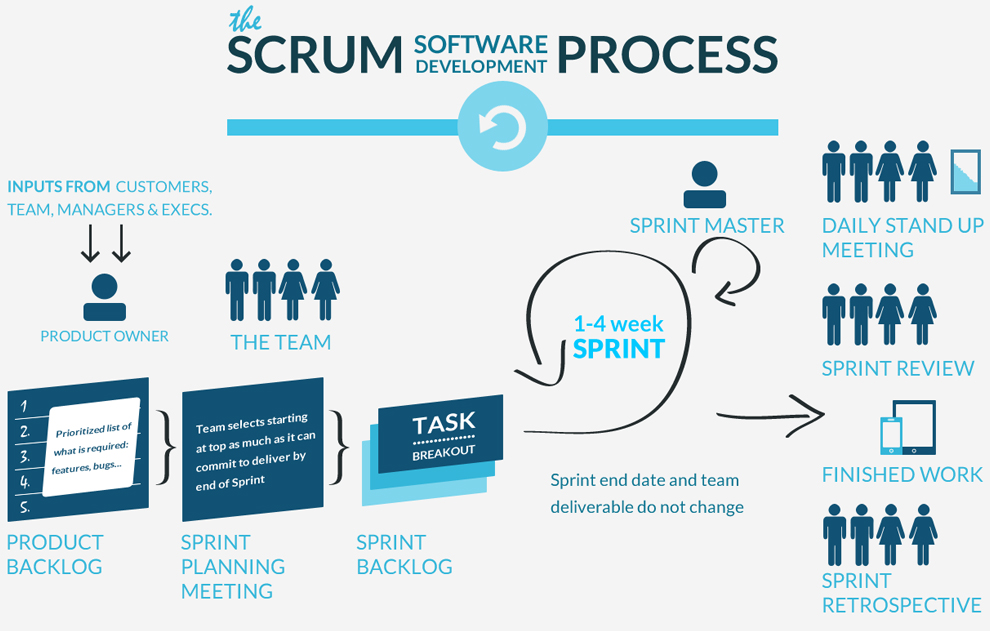
\includegraphics[scale=0.35]{immagini/processo/Scrum.jpg}
	\caption{\textit{Processo di sviluppo Scrum}}
\end{figure}\FloatBarrier

\subsection{Il processo Scrum}
Il processo Scrum è stato ideato da Jeff Sutherland e Ken Schwaber nei primi anni '90, i quali lo hanno codificato e presentato nel 1995 alla conferenza OOPSLA\ped{G} (Object-Oriented Programming, System, Languages \& Applications), pubblicando "Scrum Sofware Development Process".
\\
Il nome 'Scrum', un termine riferito alla mischia nel rugby, è stato preso da un testo del 1986, \textit{'The New Product Development Game'}, scritto da Ikujiro Nonaka e Hirotaka Takeuchi, nel quale venne introdotta una prima idea dello Scrum di oggi.
\\
Nel loro testo vengono appunto evidenziate numerose analogie tra le squadre nel gioco del rugby ed i team di sviluppo nella produzione di software, spiegando come le migliori prestazioni nello sviluppo di prodotti complessi si ottengono quando ai team, considerati come piccole, indipendenti unità di persone, vengono assegnati obiettivi piuttosto che attività, dimostrando che i team migliori sono quelli che hanno la possibilità di studiare le proprie tattiche su come arrivare all'obiettivo condiviso.

\subsection{La teoria Scrum}
La teoria di Scrum si basa sul processo di controllo empirico, il quale afferma che la conoscenza scaturisce dall'esperienza e nel prendere decisioni basate su ciò che si sia, applicando quindi un approccio incrementale e iterativo per ottimizzare la prevedibilità e controllare i rischi, sfruttando tre pilastri di base:
\begin{enumerate}
	\item Trasparenza \\ Gli aspetti rilevanti del processo devono essere visibili ai responsabili del risultato dello stesso, inoltre tali aspetti devono essere definiti da uno standard comune per consentire agli osservatori di comprendere quello che vedono, per esempio un linguaggio comune per riferirsi al processo e una definizione comune per il termine del processo.
	\item Ispezione \\ Gli utilizzatori di Scrum devono frequentemente analizzare gli artefatti prodotti ed i progressi ottenuti per il conseguimento degli obiettivi preposti, per identificare variazioni inaspettate. Tali verifiche non devono essere troppo frequenti e sono più utili se effettuate da appositi ispettori nel posto di lavoro.
	\item Adattamento \\ Se un ispettore determina che uno o più aspetti di un processo deviano dai limiti accettabili, deve essere eseguito quanto prima un aggiustamento, per minimizzare future deviazioni.
\end{enumerate}

\subsection{Ruoli Scrum}
\subsubsection{Product Owner}
Il product Owner rappresenta gli stakeholder\ped{G} ed ha il ruolo di massimizzare il valore del prodotto del Team di Sviluppo, definendo i requisiti del prodotto e la loro priorità, aggiungendoli al Product Backlog. Il product Owner è necessario per un team Scrum e si raccomanda che non sia combinato con il ruolo di Scrum Master.
\subsubsection{Scrum Master}
Lo Scrum Master fa in modo che Scrum sia compreso e messo in atto, assicurandosi che il Team di Sviluppo aderisca alla teoria, alle pratiche e alle regole Scrum, facendo in modo che, anche gli operatori esterni al team Scrum, capiscano quali iterazioni aiutino il team e quali siano dannose, massimizzando il valore creato dal team.
\subsubsection{Team di Sviluppo}
Il Team di Sviluppo consiste in un piccolo numero di professionisti che si occupano di creare gli incrementi che portano al raggiungimento dell'obiettivo della Sprint.
\\
La dimensione di un Team di Sviluppo solitamente è fra tre e i nove membri; poiché averne meno di tre riduce di troppo l'iterazione tra i membri ed averne più di nove aumenta eccessivamente la complessità di gestione.
\subsubsection{Artefatti Scrum}
Gli Artefatti Scrum rappresentano metodi per ottenere trasparenza ed opportunità di ispezione e adattamento, creati per massimizzare la trasparenza dei valori chiave, facendo in modo che tutti abbiano ua piena conoscenza dell'artefatto.
\subsubsection{Product Backlog}
Il Product Backlog è una lista ordinata di tutto ciò che può essere utile riguardo al prodotto e viene utilizzato come unica fonte di requisiti per qualsiasi cambiamento da apportare; il Product Owner è responsabile di mantenere aggiornato il Product Backlog in tutti i suoi aspetti, sia nel contenuto che nell'ordinamento.
\\
Il Product Backlog non è mai completo, in quanto comprende una lista che evolve dinamicamente con lo sviluppo del prodotto, identificando quali sono le caratteristiche che il prodotto deve avere per essere appropriato, utile e competitivo.
\\
Nel Product Backlog sono riportate tutte le funzionalità, i requisiti, i miglioramenti e le correzioni che costituiscono tutti i cambiamenti che devono essere effettuati al prodotto in rilasci futuri, gli oggetti nel Product Backlog sono tutti dotati di una descrizione, una priorità ed un valore che ne definisce lo sforzo previsto per apportare la modifica.
\\
Oggetti con priorità più alta sono solitamente meglio descritti che quelli con priorità bassa, per aiutare il Team di Sviluppo a concentrarsi sui cambiamenti più impellenti.
\subsection{La Sprint}
Il cuore di Scrum sono le Sprint: si tratta di un'unità di tempo, la cui durata può variare da una settimana ad un mese, durante la quale viene creato un incremento di prodotto utilizzabile e potenzialmente rilasciabile. In ciascuna Sprint si definisce lo scopo da raggiungere ed un piano che aiuti nello sviluppo, viene realizzato il lavoro di sviluppo ed il prodotto risultante.
\\
Le Sprint possono essere cancellate unicamente dal Product Owner, solitamente quando non ha più senso proseguire a causa di mutamenti di direzione dell'azienda, del mercato o delle tecnologie che ne rendano obsoleto l'obiettivo.
\\
Le attività che definiscono il lavoro di una Sprint consistono in:
\begin{itemize}
	\item \textbf{Pianificazione della Sprint} \\
	Nella fase di Pianificazione della Sprint tutto il team Scrum collabora per definire l'obiettivo generale basandosi principalmente sul Product Backlog, sull'ultimo incremento del prodotto, sulla previsione della capacità del Team di Sviluppo sulle loro prestazioni passate, aiutando a specificare cosa può essere fatto durante la Sprint e le modalità per ottenere l'incremento desiderato.
	\item \textbf{Scrum Giornalieri} \\
	Gli Scrum Giornalieri sono dei brevi incontri, di circa quindici minuti, del Team di Sviluppo per sincronizzare le proprie attività; ogni membro del team spiega cosa ha realizzato nel giorno precedente, cosa considera di fare nel giorno corrente e se ha riscontrato difficoltà impreviste che possono impedire o rallentare il raggiungimento dell'obiettivo predefinito. Gli Scrum Giornalieri sono utilizzati per valutare i progressi verso l'obiettivo della Sprint di volta in volta e per definire efficacemente le prestazioni del Team di Sviluppo.
	\item \textbf{Revisione Sprint} \\
	Nella revisione della Sprint si analizza l'incremento ottenuto e si aggiorna il Product Backlog, se necessario, collaborando con gli stakeholders per definire come ottimizzare il valore degli incrementi.
	\\
	La Revisione Sprint è un incontro informale e la presentazione dell'incremento punta a sollecitare i feedback e ad aumentare la collaborazione tra le parti.
	\\
	Solitamente una Revisione Sprint dura quattro ore per Sprint di un mese, mentre può durare meno in casi di Sprint più brevi, a discrezione dello Scrum Master.
	\item \textbf{Retrospettiva Sprint} \\
	La Retrospettiva Sprint avviene subito dopo la Revisione e prima della nuova Pianificazione ed è utilizzata dal team Scrum per ispezionare il proprio lavoro, individuando come sono progredite le attività assegnate, identificare quali sono state le problematiche più importanti e pianificare metodi per migliorare le modalità di lavoro del team.
	\\
	LA Retrospettiva Sprint dura al massimo tre ore, secondo la durata della Sprint
\end{itemize}

Nei suoi processi di sviluppo software ASi adotta la metodologia Scrum, che fornisce strumenti particolarmente adeguati alle proprie modalità di rapportarsi con i clienti, garantendo affidabilità nelle tempistiche e nelle personalizzazioni, nonché le opportune interazioni con gli stakeholders.
\\
La suddivisione del lavoro in Sprint definisce, infatti, con buona precisione, i tempi di sviluppo e consente, grazie alla breve durata di ogni Sprint, di migliorare l'andamento del lavoro per meglio confrontarsi alle richieste del cliente.
\\
Le revisioni previste da ogni Sprint impongono inoltre un confronto diretto con i committenti, favorendo la definizione delle loro esigenze e precisando i requisiti da soddisfare nelle Sprint future.
\\
La metodologia Scrum, che prevede di ottenere sempre un incremento funzionale al termine di ogni Sprint, favorisce pertanto l'applicazione di correzioni o integrazioni puntuali a progetti già avviati, ottenendo il progressivo affinamento dei prodotti della suite Plain, sia per quelli in fase di sviluppo, sia per quelli già rilasciati.

\subsection{Tecnologie usate dall'azienda}
\subsubsection{.NET}

\begin{figure}[ht]
	\centering
	
\includegraphics[scale=0.40]{immagini/processo/DotNet.jpg}
	\caption{\textit{Funzionalità versioni .NET}}
\end{figure}\FloatBarrier

ASI, essendo una consolidata partner Microsoft, sfrutta come base per lo sviluppo dei suoi progetti la tecnologia .NET di Microsoft, la quale è una piattaforma di sviluppo software indicata per la programmazione ad oggetti, sviluppata da Microsoft come contrapposizione al linguaggio Java.
\\
Diffusa la prima volta nel 2002, .NET ottenne subito un vantaggio su Java diventando standard ISO nel 2003 (ISO 23270 ed ISO 23271) ed avendo come caratteristica di essere indipendente dalla versione di Windows su cui è installata.
\\
.NET è un'implementazione della CLI (Common Language Infrastructure), una specifica che definisce un ambiente che permette a più linguaggi di alto livello di essere utilizzati su differenti piattaforme senza la necessità di essere riscritto.
\\
.NET infatti contiene compilatori per svariati linguaggi forniti da Microsoft (C\#, Visual Basic .NET, JAvaScript, J\#, etc.) e consente di utilizzare altri linguaggi tramite compilatori forniti da produttori di terzi, che traducano il linguaggio di alto livello scelto in CIL (Common Intermediate Language), il linguaggio di livello più basso previsto dalla piattaforma .NET e della CLI, che svolge lo stesso ruolo del Bytecode in Java.
\\
Il CIL è un linguaggio assembly orientato agli oggetti completamente basato su stack.

\begin{figure}[ht]
	\centering
	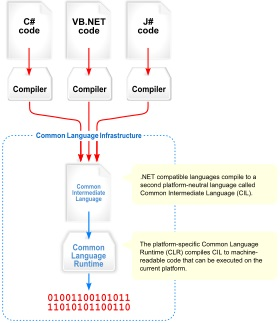
\includegraphics[scale=0.90]{immagini/processo/CIL.jpg}
	\caption{\textit{Schema Common Language Infrastructure}}
\end{figure}\FloatBarrier

il CLI viene eseguito a Runtime\ped{G} dalla CLR (Common Language Runtime), che rappresenta sia la macchina virtuale di Microsoft, sia le librerie standard della piattaforma .NET.
\\
All'interno dell CLR è presente il CLS (Common Language Specification), un ambiente di esecuzione usato principalmente sui sistemi operativi Microsoft, che i compilatori devono supportare per permettere l'interoperabilità tra i diversi linguaggi di programmazione.
\\
Esistono anche implementazioni per sistemi Unix\ped{G} e Linux\ped{G}, la più famosa denominata Mono è un'implementazione multi-piattaforma del CLS.

\subsubsection{Visual Studio}
Visual Studio è un IDE\ped{G} (Integrated Development Environment) sviluppato da Microsoft per aiutare lo sviluppo di programmi che utilizzano .NET, supportando diversi tipi di linguaggio (C,C++,C\#,F\#,Visual Basic .NET, etc), contenendo un compilatore .NET per tutti i linguaggi supportati, traducendoli in IL (Intermediate Language).
\\
Visual Studio eredita dal suo predecessore, Visual Basic, la tecnologia IntelliSense, che permette di correggere errori sintattici e alcuni logici senza effettuare una compilazione, facilitando la scrittura del codice. Possiede anche un debugger interno per il rilevamento e correzione di errori logici a runtime e fornisce doversi strumenti per l'analisi prestazionale.
\\
Una delle caratteristiche che ha portato ASI ad utilizzare Visual Studio, oltre ad essere l'IDE predefinito per lo sviluppo .NET, è la sua integrazione nativa con l'ambiente di sviluppo di gruppo Team Fondation Server.

\subsubsection{Team Fondation Server}
Team Fondation Server (p TFS) è un set di strumenti per incrementare la collaborazione tra sviluppatori indipendentemente dal linguaggio utilizzato. Tali strumenti interagiscono con l'IDE scelto e sono integrati automaticamente in Visual Studio, aiutando con il controllo della versione, fornendo repository\ped{G} privati per gestire il codice senza dover uscire dall'IDE, con l'integrazione continua, consentendo di compilare e testare la qualità delle applicazioni prodotte dopo ogni modifica, aiutando la distribuzione automatica dei prodotti che superano i test.
\\
Le funzionalità di TFS più utilizzate da ASI forniscono strumenti con Visual Studio per l'implementazione della metodologia Scrum nello sviluppo del prodotto, fornendo svariati strumenti per definire in un modo semplice ed intuitivo il lavoro da svolgere.
\\
TFS fornisce innanzitutto una visualizzazione del Product Backlog per il progetto, dove è possibile visualizzare, inserire e modificare in modo intuitivo gli oggetti nel Product Backlog, ai quali è possibile definire un ampio numero di specifiche, semplificando di molto la creazione e gestione di questo importante artefatto della metodologia Scrum.
\\
TFS consente di pianificare le Sprint da effettuare semplicemente definendo le date di inizio e fine delle stesse, rendendo chiaro il numero di incrementi da apportare e le tempistiche da eseguire. Alle Sprint è poi possibile inserire oggetti del Product Backlog, per precisare gli incrementi che si svolgeranno in quel tempo e per definire la quantità di sforzo necessaria per portare a termine la sprint.
\\
E'possibile inoltre definire i profili utente del Team di Sviluppo, inserendo la quantità di sforzo giornaliero che possono impiegare durante li sprint, il ruolo che ricoprono ed i loro giorno lavorativi, in modo da ottenere in modo semplice la quantità di sforzo applicabile dal Team di Sviluppo nella Sprint che si va a definire. Dopo aver inserito gli oggetti del Product Backlog nella Sprint è possibile collegarli direttamente ai membri del Team di Sviluppo interessati, ottenendo un immediato schema dello sforzo richiesto da ogni membro del Team, consentendo poi di redistribuire gli oggetti in modo che lo sforzo di ogni membro sia utilizzato al massimo dell'efficacia.
\\
Il TFS aiuta a rendere chiaro e intuitivo lo svolgimento del lavoro da parte del Team di Sviluppo a tutti i ruoli interessati ed aiuta i nuovi utenti ad implementare facilmente la metodologia Scrum nel loro progetto.

\section{Scrum in ASI}
Il Team di Sviluppo ASI non ha personalizzato l'approccio a Scrum in alcun modo, il ruolo di Product Owner è stato dato ad uno dei membri fondatori dell'azienda, il quale ha creato il Product Backlog per ogni progetto in corso, gli oggetti al suo interno sono stati definiti 'Task' ed hanno utilizzato la definizione che TFS fornisce per determinare il termine.
\\
Per la gestione delle richieste al Team di Sviluppo da parte degli altri dipendenti dell'azienda, lo Scrum Master ha imposto che venissero inviate tramite inserimento di Task nel relativo progetto a cui la richiesta fa capo, lasciando che fosse il Product Owner poi ad impostarne la priorità per meglio guidare il lavoro degli sviluppatori.
\\
Le Sprint in ASI sono sempre della durata settimanale (10 giorni lavorativi), effettuando solitamente la fase di Revisione e Retrospettiva il lunedì e la fase di Pianificazione della Sprint successiva il martedì.

\section{Obiettivi dello Stage}
L'obiettivo dello stage era la creazione di un applicativo mobile, multi-piattaforma, che permetta la generazione di rapportini firmabili, tramite firma biometrica, in formato pdf.
\\
Mi è stato richiesto inoltre di sviluppare dei servizi che espongono i dati necessari all'applicazione e di realizzare una sincronizzazione intelligente dei dati, dove ciò che transita è solo ciò che effettivamente è stato modificato. 
\\
Per la realizzazione dell'applicazione cross-platform mi è stato richiesto l'uso del framework \textbf{Xamarin.Forms}, un framework per lo sviluppo multi-piattaforma che fornisce varie API per l'applicazione della CLI negli applicativi mobili sfruttando il framework .NET, e consente sopratutto di sviluppare UI\ped{G} (User Interfaces) che possono essere condivise tra dispositivi Android, iOS e Windows Phone, traducendo a runtime il codice condiviso in codice nativo.

\begin{figure}[ht]
	\centering
	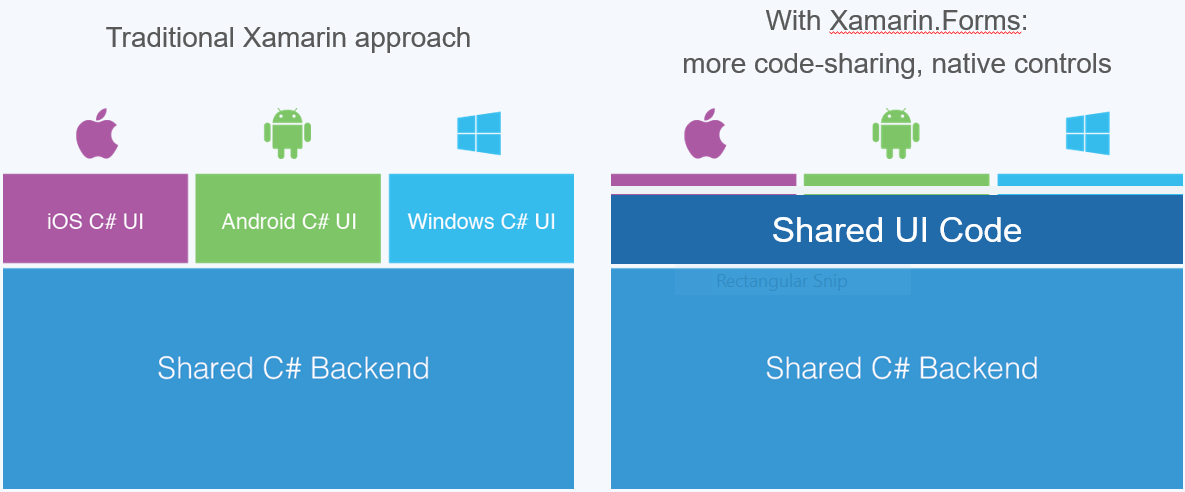
\includegraphics[scale=0.57]{immagini/processo/xamarinForms.png}
	\caption{\textit{Differenza di approccio tra Xamarin e Xamarin.Forms}}
\end{figure}\FloatBarrier

Mi è stato richiesto anche di valutare alcuni modi per gestire la realizzazione di un pdf esclusivamente nel dispositivo mobile a partire da un template\ped{G}, senza creare il documento direttamente via codice. Questa scelta è stata accordata per garantire una elevata manutenibilità del software, che in caso di variazioni del rapportino da emettere, rende semplice la modifica del template.
\\
Sono state valutate varie librerie commerciali per la generazione del pdf a partire da un template, ma nessuna offriva realmente ciò che interessava all'azienda, pertanto si è deciso di puntare in un template XSLT che a partire da un XML con associato un foglio di stile, permette la generazione di una pagina HTML che a sua volta sarà convertita in pdf grazie alle funzionalità offerte da pacchetto iTextSharp.

\subsection{Vincoli del progetto di stage}
Una volta inserito come membro del Team di sviluppo di ASI, mi è stato chiesto di seguire le direttive di sviluppo dei software aziendali, che si ricollegano alle norme di scrittura del codice definite da Microsoft per lo sviluppo .NET.

\subsection{Impostazione del lavoro}
Il lavoro da svolgere durante lo stage è suddiviso in \textbf{fasi},che sono state introdotte in varie Task dal tutor aziendale ed assegnate di volta in volta al mio profilo dallo Scrum Master del Team di sviluppo, alla Pianificazione di ogni Sprint.
\begin{itemize}
	\item[I.] La prima fase è stata dedicata alle conoscenze generali per approfondire le conoscenze del .NET Framework 4.5 e familiarizzare con gli strumenti integrati in Visual Studio, quali TFS, Testing e Continuous integration.
	\item[II.] La seconda fase è stata dedicata all'acquisizione degli standard aziendali, la lettura del manuale di sviluppo contenente le direttive imposte per la coerenza dell'interfaccia grafica e l'architettura delle applicazioni Plain.
	\item[III.] La terza fase è stata dedicata alla formazione sugli strumenti e sui metodi per raggiungere gli obiettivi fissati. Durante questa periodo formativo ho appreso l'utilizzo di Xamarin.Forms e analizzato i vari metodi per la generazione di documenti elettronici in formato pdf nei dispositivi mobile.
	\item[VI.] La quarta fase è stata dedicata all'analisi dei requisiti dell'applicativo da produrre, durante il quale ho effettuato delle riunioni con il tutor aziendale ed il committente per affinare la lista dei requisiti del prodotto.
	\item[V.] La quinta fase è stata dedicata allo sviluppo del progetto, iniziato con una attività di progettazione e proseguita dalla codifica, suddivisa a sua volta in varie Task per coprire tutte le aree dell'applicativo da sviluppare. 
	\item[VI.] La Sesta fase è stata utilizzata per redigere la documentazione del prodotto.
\end{itemize}









